\begin{myTheorem}[Dominance of the sector areas in the outer band]  
Given a unit disk with a radial partition of $n\ge2$ bands, and two integers $k$ and $j$ such that $1\le k < j \le n$.
  % = =  e q u a t i o n
  \begin{equation}
    A_{11} > A_{22} > \dots > A_{nn} > 0
  \end{equation}
  % = =
\end{myTheorem}  %  -  -  -  -  -  -  -  -  -  -  -  -  -  -  -  -
\begin{proof}  %  +  +  +  +  +  +  +  +  +  +  +  +  +  +  +  +
We employ a Matryoshka doll strategy by nesting the areas as shown in figure \eqref{fig:Matryoshka}.
\begin{figure}[htbp] %  figure placement: here, top, bottom, or page
   \centering
   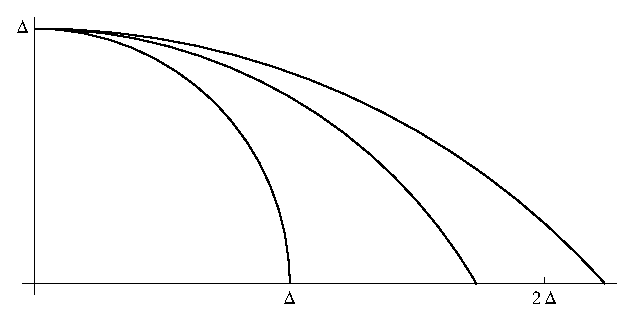
\includegraphics[ width = 3in ]{graphics/Matryoshka.eps} 
   \caption{Nesting the areas of interest. This is the family of curves in \eqref{eq:Matryoshka} for $k=1,2,3$.}
   \label{fig:Matryoshka}
\end{figure}
The equation for curve $y_{k}(x)$ is
  % = =  e q u a t i o n
  \begin{equation}
    y_{k}(x) = \sqrt{(k \Delta)^{2} - x^{2}} - (k-1)\Delta, \quad 0\le x \le \sqrt{2k-1} .
    \label{eq:Matryoshka}
  \end{equation}
  % = =
Over this domain the curve $y\ge0$. For the proof it is sufficient to show dominance over the domain of the subsumed curve. Given integers $j$ and $k$ such that $1\le j < k \le n$ one must prove that
  % = =  e q u a t i o n
  \begin{equation}
    y_{k}(x) \ge y_{j}(x), \qquad 0\le x \le \sqrt{2k-1} .
    \label{eq:yk gt yj}
  \end{equation}
  % = =
By subtracting the Maclauren expansions we find
  % = =  e q u a t i o n
  \begin{equation}
  \begin{split}
    y_{k}(x) - y_{j}(x) 
      & = \sum_{m=1}^{\infty} \binom{1/2}{m} \frac{x^{2m}}{\Delta^{2m-1}}\paren{\frac{1}{j^{2m-1}}-\frac{1}{k^{2m-1}}} \\
      & \approx 
      \frac{x^{2}}{2\Delta}\paren{\frac{1}{j}-\frac{1}{k}} 
    + \frac{x^{4}}{8\Delta^{3}}\paren{\frac{1}{j^{3}}-\frac{1}{k^{3}}} 
    + \frac{x^{6}}{16 \Delta^{5}} \paren{\frac{1}{j^{5}}-\frac{1}{k^{5}}} 
    + \frac{5x^{8}}{128 \Delta^{7}} \paren{\frac{1}{j^{7}}-\frac{1}{k^{7}}} 
    + \dots 
  \end{split}
  \end{equation}
  % = =
All these terms are positive which establishes \eqref{eq:yk gt yj}.
\end{proof}  %  +  +  +  +  +  +  +  +  +  +  +  +  +  +  +  +

\endinput %-------------------------------